\section{Aufgabe E5}
Gegeben sei die Kontingenztafel f�r die Merkmale X Baumart (Ulme, Kiefer, Fichte) und Y Sch�dlingsbefall
durch Borkenk�fer (kein, gering, mittel, gro�)

\begin{figure}[!htbp]
\centering
\fbox{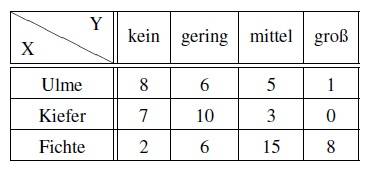
\includegraphics[width=0.6\linewidth]{./chapters/Grafiken_TB/TB_E5.jpg}}
\end{figure}
\subsection{Berechnen Sie die Randverteilungen in Wahrscheinlichkeiten}
\vspace{9cm}

\subsection{Man bestimme die bedingte Verteilung von Y bedingt auf X =Ulme.}
\vspace{2cm}

\subsection{Sind die Merkmale unabh�ngig? }


